\documentclass[sigconf]{acmart}

\usepackage{amsmath}
\usepackage{amssymb}
\usepackage[english]{babel}
\usepackage{csquotes} % displayquote environment
\usepackage{microtype}
\usepackage{tikz}
\usetikzlibrary{arrows.meta}

\hyphenation{time-stamp time-stamps time-stamped}

\copyrightyear{2019}
\acmYear{2019}
\setcopyright{rightsretained}
\acmConference[]{---}{---}{---}
%\acmBooktitle{}
%\acmPrice{15.00}
%\acmDOI{}
%\acmISBN{}

\begin{document}
\title{Interleaving anomalies in collaborative text editors}

\author{Martin Kleppmann}
\email{mk428@cl.cam.ac.uk}
\orcid{0000-0001-7252-6958}
\affiliation{%
  \institution{University of Cambridge, UK}
  %\streetaddress{William Gates Building, 15 JJ Thomson Avenue}
  %\city{Cambridge}
  %\state{}
  %\postcode{CB3 0FD}
  %\country{UK}
}

\author{Victor B.\ F.\ Gomes}
\email{vb358@cl.cam.ac.uk}
\orcid{0000-0002-2954-4648}
\affiliation{%
  \institution{University of Cambridge, UK}
  %\streetaddress{William Gates Building, 15 JJ Thomson Avenue}
  %\city{Cambridge}
  %\state{}
  %\postcode{CB3 0FD}
  %\country{UK}
}

\author{Dominic P.\ Mulligan}
\email{Dominic.Mulligan@arm.com}
\orcid{0000-0003-4643-3541}
\affiliation{%
  \institution{Arm Research, UK}
  %\streetaddress{110 Fulbourn Road}
  %\city{Cambridge}
  %\state{}
  %\postcode{CB1 9NJ}
  %\country{UK}
}

\author{Alastair R.\ Beresford}
\email{arb33@cl.cam.ac.uk}
\orcid{0000-0003-0818-6535}
\affiliation{%
  \institution{University of Cambridge, UK}
  %\streetaddress{William Gates Building, 15 JJ Thomson Avenue}
  %\city{Cambridge}
  %\state{}
  %\postcode{CB3 0FD}
  %\country{UK}
}

\begin{abstract}
Collaborative text editors allow two or more users to concurrently edit a shared document without merge conflicts.
Such systems require an algorithm to provide \emph{convergence}, ensuring all clients that have seen the same set of document edits are in the same state.
Unfortunately convergence alone does not guarantee that a collaborative text editor is usable.
Several published algorithms for collaborative text editing exhibit an undesirable anomaly in which concurrently inserted portions of text with a well-defined order may be randomly interleaved on a character-by-character basis, resulting in an unreadable jumble of letters.
Although this anomaly appears to be known informally by some researchers in the field, we are not aware of any published work that fully explains or addresses it.
We show that several algorithms suffer from this problem, explain its cause, and also identify a lesser variant of the anomaly that occurs in another algorithm.
Moreover, we propose a specification of collaborative text editing that rules out the anomaly, and show how to prevent the lesser anomaly from occurring in one particular algorithm.
\end{abstract}

% The code below is generated by the tool at http://dl.acm.org/ccs.cfm.
\begin{CCSXML}
<ccs2012>
<concept>
<concept_id>10003752.10003809.10010172</concept_id>
<concept_desc>Theory of computation~Distributed algorithms</concept_desc>
<concept_significance>500</concept_significance>
</concept>
<concept>
<concept_id>10011007.10010940.10010992.10010993.10010996</concept_id>
<concept_desc>Software and its engineering~Consistency</concept_desc>
<concept_significance>500</concept_significance>
</concept>
<concept>
<concept_id>10003120.10003130.10003233</concept_id>
<concept_desc>Human-centered computing~Collaborative and social computing systems and tools</concept_desc>
<concept_significance>300</concept_significance>
</concept>
<concept>
<concept_id>10003456.10003457.10003567.10003570</concept_id>
<concept_desc>Social and professional topics~Computer supported cooperative work</concept_desc>
<concept_significance>300</concept_significance>
</concept>
<concept>
<concept_id>10010520.10010521.10010537</concept_id>
<concept_desc>Computer systems organization~Distributed architectures</concept_desc>
<concept_significance>300</concept_significance>
</concept>
</ccs2012>
\end{CCSXML}

\ccsdesc[500]{Theory of computation~Distributed algorithms}
\ccsdesc[500]{Software and its engineering~Consistency}
\ccsdesc[300]{Human-centered computing~Collaborative and social computing systems and tools}
\ccsdesc[300]{Social and professional topics~Computer supported cooperative work}
\ccsdesc[300]{Computer systems organization~Distributed architectures}

\keywords{CRDTs, collaborative text editing, specification, consistency}
\maketitle

\section{Introduction}

In collaborative software, several users may contribute to a project by creating and editing shared documents such as text documents, spreadsheets, or similar.
When a user wishes to view a document, a copy of that document is loaded on the user's computer in a web-browser tab, or in a native app on their device.
Any changes made by the user are immediately applied to the local copy of the document on the user's computer, and then asynchronously sent to any other users who have a copy of the document---possibly via a server, which may also store a copy.
This collaboration scenario is very similar to the problem of replication in distributed databases: in this context, the shared data is a database rather than a document, and each node that has a copy of the data is called a \emph{replica}.

At a high level, there are two possible ways of managing modifications to documents: either the system enforces that only one user at a time may edit a particular document using a synchronization mechanism (e.g. locks), or the system allows multiple users to edit a document concurrently.
This latter case is known as \emph{optimistic replication}~\cite{Saito:2005jw}.
In an optimistic replication setting, several users may make changes at the same time, causing the state of these users' documents to diverge.
This is illustrated in Figure~\ref{fig:hello-world}, where one user changes the text of their document from \texttt{`Hello!'} to \texttt{`Hello World!'}, while another user concurrently edits the text of their document to read \texttt{`Hello! :)'}.
In order to ensure that no user input is lost, these concurrent changes must be \emph{merged} into a consistent document---in this example \texttt{`Hello World! :)'}.

\begin{figure*}[p]
  \centering
  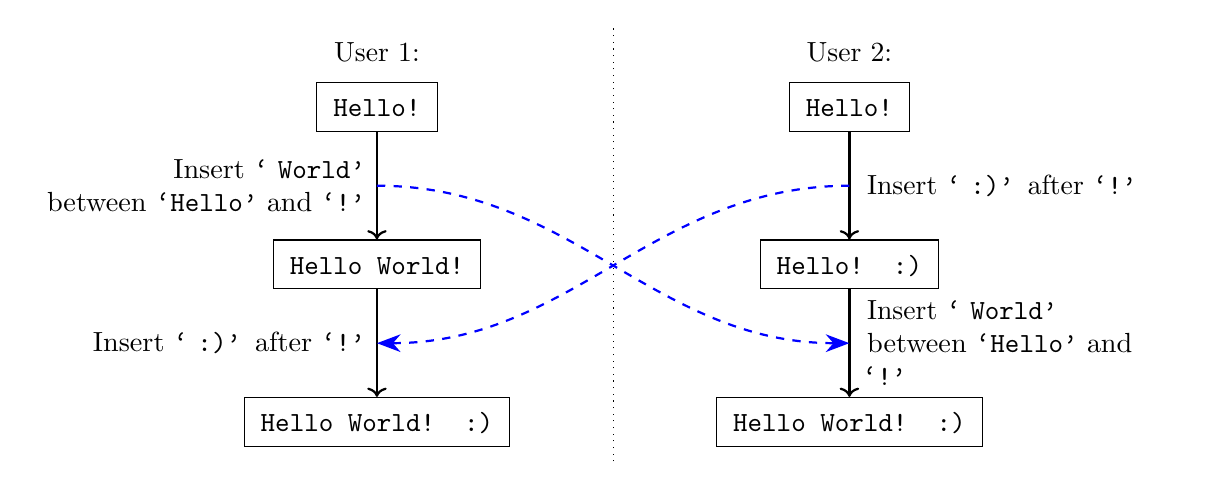
\begin{tikzpicture}[auto,scale=1.0]
    \tikzstyle{box}=[rectangle,draw,inner xsep=6pt,text height=9pt,text depth=2pt]
	\tikzstyle{leftevent}=[left,inner xsep=6pt,text width=4cm,text ragged left,midway]
	\tikzstyle{rightevent}=[right,inner xsep=6pt,text width=4cm,text ragged,midway]
	\tikzstyle{time}=[thick,->]
	\tikzstyle{network}=[thick,dashed,blue,-{Stealth[length=3mm]}]
	\node (left0)  at (0,4.7) {User 1:};
	\node (left1)  at (0,4.0) [box] {\texttt{Hello!}};
	\node (left2)  at (0,2.0) [box] {\texttt{Hello World!}};
	\node (left3)  at (0,0.0) [box] {\texttt{Hello World! :)}};
	\node (right0) at (6,4.7) {User 2:};
	\node (right1) at (6,4.0) [box] {\texttt{Hello!}};
	\node (right2) at (6,2.0) [box] {\texttt{Hello! :)}};
	\node (right3) at (6,0.0) [box] {\texttt{Hello World! :)}};
	\draw [time] (left1)  -- (left2)  node (send1) [leftevent]  {Insert \texttt{`~World'}\\between \texttt{`Hello'} and \texttt{`!'}};
	\draw [time] (right1) -- (right2) node (send2) [rightevent] {Insert \texttt{` :)'} after \texttt{`!'}};
    \draw [time] (left2)  -- (left3)  node (recv2) [leftevent]  {Insert \texttt{` :)'} after \texttt{`!'}};
    \draw [time] (right2) -- (right3) node (recv1) [rightevent] {Insert \texttt{`~World'}\\between \texttt{`Hello'} and \texttt{`!'}};
    \draw [network] (send1.east) to [out=0,in=180] (recv1.west);
    \draw [network] (send2.west) to [out=180,in=0] (recv2.east);
	\path [draw,dotted] (3,-0.5) -- (3,5.0);
  \end{tikzpicture}
  \caption{Simple concurrent text editing example. Solid black lines indicate state changes over time while dashed blue arrows indicate network communication.}
  \label{fig:hello-world}
\end{figure*}

\begin{figure*}[p]
  \centering\vspace{2em}
  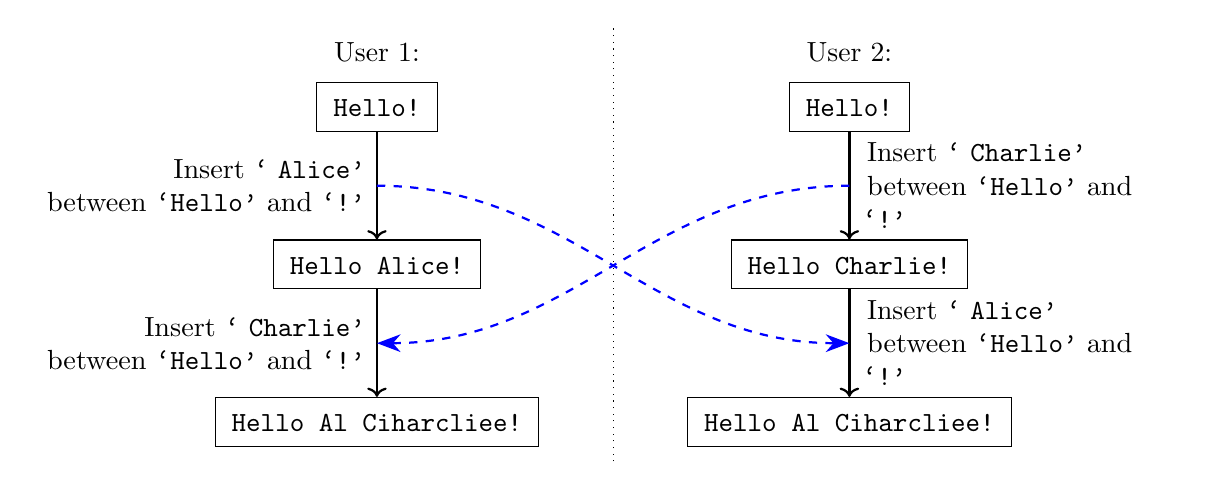
\begin{tikzpicture}[auto,scale=1.0]
    \tikzstyle{box}=[rectangle,draw,inner xsep=6pt,text height=9pt,text depth=2pt]
	\tikzstyle{leftevent}=[left,inner xsep=6pt,text width=4cm,text ragged left,midway]
	\tikzstyle{rightevent}=[right,inner xsep=6pt,text width=4cm,text ragged,midway]
	\tikzstyle{time}=[thick,->]
	\tikzstyle{network}=[thick,dashed,blue,-{Stealth[length=3mm]}]
	\node (left0)  at (0,4.7) {User 1:};
	\node (left1)  at (0,4.0) [box] {\texttt{Hello!}};
	\node (left2)  at (0,2.0) [box] {\texttt{Hello Alice!}};
	\node (left3)  at (0,0.0) [box] {\texttt{Hello Al Ciharcliee!}};
	\node (right0) at (6,4.7) {User 2:};
	\node (right1) at (6,4.0) [box] {\texttt{Hello!}};
	\node (right2) at (6,2.0) [box] {\texttt{Hello Charlie!}};
	\node (right3) at (6,0.0) [box] {\texttt{Hello Al Ciharcliee!}};
	\draw [time] (left1)  -- (left2)  node (send1) [leftevent]  {Insert \texttt{`~Alice'}\\between \texttt{`Hello'} and \texttt{`!'}};
	\draw [time] (right1) -- (right2) node (send2) [rightevent] {Insert \texttt{`~Charlie'}\\between \texttt{`Hello'} and \texttt{`!'}};
    \draw [time] (left2)  -- (left3)  node (recv2) [leftevent]  {Insert \texttt{`~Charlie'}\\between \texttt{`Hello'} and \texttt{`!'}};
    \draw [time] (right2) -- (right3) node (recv1) [rightevent] {Insert \texttt{`~Alice'}\\between \texttt{`Hello'} and \texttt{`!'}};
    \draw [network] (send1.east) to [out=0,in=180] (recv1.west);
    \draw [network] (send2.west) to [out=180,in=0] (recv2.east);
	\path [draw,dotted] (3,-0.5) -- (3,5.0);
  \end{tikzpicture}
  \caption{Two concurrent insertions at the same position are interleaved.}
  \label{fig:bad-merge}
\end{figure*}

\begin{figure*}[p]
  \centering\vspace{2em}
  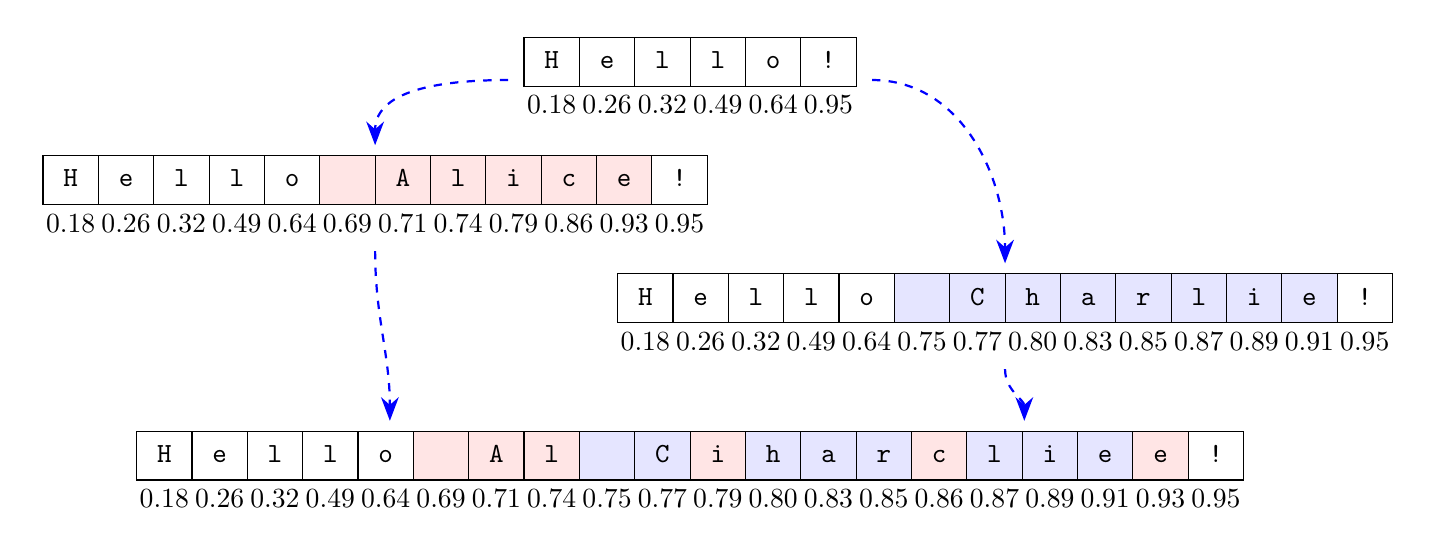
\begin{tikzpicture}[auto,scale=1.0]
    \tikzstyle{box}=[rectangle,draw,inner xsep=6pt,text height=9pt,text depth=2pt]
	\tikzstyle{state}=[matrix,column sep={20pt,between origins}]
	\tikzstyle{val}=[draw,anchor=base,minimum width=20pt,text height=8pt,text depth=3pt]
	\tikzstyle{oid}=[anchor=base]
	\tikzstyle{ins1}=[fill=red!10]
	\tikzstyle{ins2}=[fill=blue!10]
	\tikzstyle{leftevent}=[left,inner xsep=6pt,text width=4cm,text ragged left,midway]
	\tikzstyle{rightevent}=[right,inner xsep=6pt,text width=4cm,text ragged,midway]
	\tikzstyle{time}=[thick,->]
	\tikzstyle{network}=[thick,dashed,blue,-{Stealth[length=3mm]}]
	\node (hello) at (4,5) [state] {
		\node [val] {\texttt{H}}; &
		\node [val] {\texttt{e}}; &
		\node [val] {\texttt{l}}; &
		\node [val] {\texttt{l}}; &
		\node [val] {\texttt{o}}; &
		\node [val] {\texttt{!}}; \\
		\node [oid] {0.18}; & % H
		\node [oid] {0.26}; & % e
		\node [oid] {0.32}; & % l
		\node [oid] {0.49}; & % l
		\node [oid] {0.64}; & % o
		\node [oid] {0.95}; \\ % !
	};
	\node (alice) at (0,3.5) [state] {
		\node [val] {\texttt{H}}; &
		\node [val] {\texttt{e}}; &
		\node [val] {\texttt{l}}; &
		\node [val] {\texttt{l}}; &
		\node [val] {\texttt{o}}; &
		\node [val,ins1] {\texttt{ }}; &
		\node [val,ins1] {\texttt{A}}; &
		\node [val,ins1] {\texttt{l}}; &
		\node [val,ins1] {\texttt{i}}; &
		\node [val,ins1] {\texttt{c}}; &
		\node [val,ins1] {\texttt{e}}; &
		\node [val] {\texttt{!}}; \\
		\node [oid] {0.18}; & % H
		\node [oid] {0.26}; & % e
		\node [oid] {0.32}; & % l
		\node [oid] {0.49}; & % l
		\node [oid] {0.64}; & % o
		\node [oid] {0.69}; & %
		\node [oid] {0.71}; & % A
		\node [oid] {0.74}; & % l
		\node [oid] {0.79}; & % i
		\node [oid] {0.86}; & % c
		\node [oid] {0.93}; & % e
		\node [oid] {0.95}; \\ % !
	};
	\node (charlie) at (8,2) [state] {
		\node [val] {\texttt{H}}; &
		\node [val] {\texttt{e}}; &
		\node [val] {\texttt{l}}; &
		\node [val] {\texttt{l}}; &
		\node [val] {\texttt{o}}; &
		\node [val,ins2] {\texttt{ }}; &
		\node [val,ins2] {\texttt{C}}; &
		\node [val,ins2] {\texttt{h}}; &
		\node [val,ins2] {\texttt{a}}; &
		\node [val,ins2] {\texttt{r}}; &
		\node [val,ins2] {\texttt{l}}; &
		\node [val,ins2] {\texttt{i}}; &
		\node [val,ins2] {\texttt{e}}; &
		\node [val] {\texttt{!}}; \\
		\node [oid] {0.18}; & % H
		\node [oid] {0.26}; & % e
		\node [oid] {0.32}; & % l
		\node [oid] {0.49}; & % l
		\node [oid] {0.64}; & % o
		\node [oid] {0.75}; & %
		\node [oid] {0.77}; & % C
		\node [oid] {0.80}; & % h
		\node [oid] {0.83}; & % a
		\node [oid] {0.85}; & % r
		\node [oid] {0.87}; & % l
		\node [oid] {0.89}; & % i
		\node [oid] {0.91}; & % e
		\node [oid] {0.95}; \\ % !
	};
	\node (interleaved) at (4,0) [state] {
		\node [val] {\texttt{H}}; &
		\node [val] {\texttt{e}}; &
		\node [val] {\texttt{l}}; &
		\node [val] {\texttt{l}}; &
		\node [val] {\texttt{o}}; &
		\node [val,ins1] {\texttt{ }}; &
		\node [val,ins1] {\texttt{A}}; &
		\node [val,ins1] {\texttt{l}}; &
		\node [val,ins2] {\texttt{ }}; &
		\node [val,ins2] {\texttt{C}}; &
		\node [val,ins1] {\texttt{i}}; &
		\node [val,ins2] {\texttt{h}}; &
		\node [val,ins2] {\texttt{a}}; &
		\node [val,ins2] {\texttt{r}}; &
		\node [val,ins1] {\texttt{c}}; &
		\node [val,ins2] {\texttt{l}}; &
		\node [val,ins2] {\texttt{i}}; &
		\node [val,ins2] {\texttt{e}}; &
		\node [val,ins1] {\texttt{e}}; &
		\node [val] {\texttt{!}}; \\
		\node [oid] {0.18}; & % H
		\node [oid] {0.26}; & % e
		\node [oid] {0.32}; & % l
		\node [oid] {0.49}; & % l
		\node [oid] {0.64}; & % o
		\node [oid] {0.69}; & %
		\node [oid] {0.71}; & % A
		\node [oid] {0.74}; & % l
		\node [oid] {0.75}; & %
		\node [oid] {0.77}; & % C
		\node [oid] {0.79}; & % i
		\node [oid] {0.80}; & % h
		\node [oid] {0.83}; & % a
		\node [oid] {0.85}; & % r
		\node [oid] {0.86}; & % c
		\node [oid] {0.87}; & % l
		\node [oid] {0.89}; & % i
		\node [oid] {0.91}; & % e
		\node [oid] {0.93}; & % e
		\node [oid] {0.95}; \\ % !
	};
	\draw [network] (hello.west)    to [out=180,in=90] (alice.north);
	\draw [network] (hello.east)    to [out=0,in=90]   (charlie.north);
	\draw [network] (alice.south)   to [out=270,in=90] (interleaved.170);
	\draw [network] (charlie.south) to [out=270,in=90] (interleaved.9);
  \end{tikzpicture}
  \caption{Interleaving due to character positions taken from a dense identifier set, e.g.\ the rational numbers $\mathbb{Q}$.}
  \label{fig:real-numbers}
\end{figure*}

Merge operations can either be performed manually---the approach used by version control systems such as \texttt{git}---or can be automated.
Conflict-free Replicated Data Types, or CRDTs~\cite{Shapiro:2011wy,Shapiro:2011un}, have been developed to automate such merges.
A CRDT is an abstract datatype whose state can be modified by performing certain operations. For example, a datatype for text editing may represent text as a list of characters, allowing characters to be inserted or deleted anywhere in the document.
Local changes are propagated to other replicas, either by encoding the updated state and merging it into remote copies of the document, or by encoding the operations and applying them to remote copies.

\subsection{Consistency for optimistic replication}

CRDTs implement a consistency model called \emph{strong eventual consistency}~\cite{Shapiro:2011un,Gomes:2017gy}, defined by the following properties:
\begin{description}
\item[Eventual delivery:] An update applied on one correct replica is eventually applied on all correct replicas.
\item[Convergence:] If the same set of updates have been applied (possibly in a different order) on two replicas then those two replicas have equivalent state.
\item[Termination:] All method executions terminate.
\end{description}
In operation-based CRDTs the convergence property is implemented by ensuring that concurrent operations \emph{commute}.
For example, consider Figure~\ref{fig:hello-world} wherein User 1 first applies the insertion of \texttt{` World'} and then applies the insertion of \texttt{` :)'} to the document, while User 2 applies the same two insertions in the opposite order.
Commutativity of the insertions ensures that the two replicas obtain the same final state.

When replicas mutually merge each others' changes, the convergence property ensures that those replicas obtain the same state.
However, we must also specify what that state should be: strong eventual consistency is necessary but it is not sufficient, as it does not capture all of the consistency properties that we require.
For example, the convergence property for a document could be met by storing all inserted characters in lexicographical order, but this does not represent a useful document editing system.
More is needed in order to ensure the system is useful.

In this paper we examine a particular consistency property for collaborative text editors that has been overlooked in the literature.
Notably, failing to satisfy this property may result in arbitrary text interleaving leading to an undesirable (garbled) document state.
We highlight existing CRDT algorithms and a specification that exhibit this anomaly, and demonstrate how to fix this flaw.

\section{The interleaving anomaly}\label{sec:anomaly}

In this section we discuss an anomaly that can lead to undesirable outcomes when two users concurrently insert text at the same position in a document.
For example, in Figure~\ref{fig:bad-merge}, two users are editing a text document that initially reads \texttt{`Hello!'}.
User 1 changes it to read \texttt{`Hello Alice!'}, while concurrently User 2 changes it to \texttt{`Hello Charlie!'}.
However, when the concurrent edits are merged, the merging algorithm randomly interleaves the two insertions of \texttt{`~Alice'} and \texttt{`~Charlie'} character by character, resulting in an unreadable jumble of characters.

Even though this outcome is obviously undesirable, it does sometimes occur in practice.
Two published CRDTs for collaborative text editing, Logoot \cite{Weiss:2009ht,Weiss:2010hx} and LSEQ \cite{Nedelec:2013ky,Nedelec:2016eo}, suffer from this problem, as we explain shortly.
In prior work~\cite{ExtendedVersion,AFP} we mechanically proved that another text editing CRDT, RGA \cite{Roh:2011dw}, does not suffer from this problem; however, RGA can exhibit a lesser variant of the anomaly, which we describe in Section~\ref{sec:lesser}.
We conjecture that Treedoc~\cite{Preguica:2009fz} and WOOT~\cite{Oster:2006wj} do not suffer from either anomaly, but we leave a rigorous proof of this claim for future work.

The reason why this anomaly occurs with Logoot and LSEQ is illustrated in Figure~\ref{fig:real-numbers}.
Conceptually, these algorithms work by assigning every character of the text a unique position identifier from a \emph{dense} ordered set; that is, for any two given identifiers we can find a new, distinct identifier that lies between the two.
The order of characters in the text is then given by the order of these identifiers.
In Figure~\ref{fig:real-numbers} we use rational numbers between 0.0 and 1.0 as identifiers.
In reality, identifiers in Logoot and LSEQ are paths through a tree, which have the same effect.

We can see in Figure~\ref{fig:real-numbers} that identifiers are assigned correctly by each of the users: the characters of \texttt{` Alice'} and \texttt{` Charlie'} are assigned rational numbers between 0.64 and 0.95 (the interval between the preceding \texttt{`Hello'} and the following \texttt{`!'}) in increasing order.
However, the exact values assigned to each character can vary arbitrarily, and since neither user knows about the other user's concurrent insertion, both users spread the identifiers of their insertions across the interval (0.64, 0.95).
When merged, the resulting character sequence is an arbitrary interleaving of the two.

We performed tests with open source implementations of Logoot \cite{AhmedNacer:2011ke,ReplicationBenchmark} and LSEQ \cite{LSEQTree,Nedelec:2016eo}, and observed this interleaving anomaly occurring in practice.
The problem is even worse if the concurrent insertions are comprised of not just a single word but a paragraph or section.
In these cases, interleaving the users' insertions would most likely result in an incomprehensible text that would have to be deleted and rewritten.

Note, however, that this problem does not occur in the example of Figure~\ref{fig:hello-world}.
Here, the merged outcome is unambiguous as the relative ordering of all parts of the text is clear: \texttt{` World'} is inserted before the exclamation mark, while the \texttt{` :)'} is inserted after it.

\subsection{Attiya et al.'s specification}\label{sec:attiya-spec}

In 2016 Attiya et al.~\cite{Attiya:2016kh} proposed $\mathcal{A}_\textsf{strong}$, an implementation-independent specification of collaborative text editing.
However, this specification also permits the interleaving anomaly; we therefore argue that it is too weak to be a suitable specification for collaborative text editing.
The definition of $\mathcal{A}_\textsf{strong}$ is as follows~\cite{Attiya:2016kh}:

\begin{displayquote}
  An abstract execution $A = (H, \textsf{vis})$ belongs to the \emph{strong list specification} $\mathcal{A}_\textsf{strong}$ if and only if there is a relation $\textsf{lo} \subseteq \textsf{elems}(A) \times \textsf{elems}(A)$, called the \emph{list order}, such that:
  \begin{enumerate}
    \item Each event $e = \mathit{do}(\mathit{op}, w) \in H$ returns a sequence of elements $w=a_0 \dots a_{n-1}$, where $a_i \in \textsf{elems}(A)$, such that
    \begin{enumerate}
      \item $w$ contains exactly the elements visible to $e$ that have been inserted, but not deleted:
	    \begin{align*}
          \quad\forall a.\; a \in w \quad\Longleftrightarrow\quad &
		  (\mathit{do}(\textsf{ins}(a, \_), \_) \le_\textsf{vis} e) \;\wedge\\ &
		  \neg(\mathit{do}(\textsf{del}(a), \_) \le_\textsf{vis} e).
		\end{align*}
      \item The order of the elements is consistent with the list order:
        \[ \forall i, j.\; (i < j) \;\Longrightarrow\; (a_i, a_j) \in \textsf{lo}. \]
      \item Elements are inserted at the specified position:
        if $\mathit{op} = \textsf{ins}(a, k)$, then $a = a_{\mathrm{min} \{k,\; n-1\}}$.
    \end{enumerate}
    \item The list order $\textsf{lo}$ is transitive, irreflexive and total, and thus determines the order of all insert operations in the execution.
  \end{enumerate}
\end{displayquote}
The list order relation $\textsf{lo}$ in this definition plays the same role as the position identifiers in Figure~\ref{fig:real-numbers}, and hence this specification permits the same interleaving anomaly.
We can correct this flaw in the $\mathcal{A}_\textsf{strong}$ specification and rule out interleaving by introducing an additional clause 1(d):

\begin{enumerate}
  \item Each event $e = \mathit{do}(\mathit{op}, w) \in H$ returns a sequence of elements $w=a_0 \dots a_{n-1}$, where $a_i \in \textsf{elems}(A)$, such that
  \begin{enumerate}
    \item \dots~(c): as before;
    \setcounter{enumii}{3}
    \item Concurrent insertions are not interleaved: that is, for any two sets of insertions $X$ and $Y$
      \begin{align*}
        X = \{x \mid \exists a.\; &x = \mathit{do}(\textsf{ins}(a, \_), \_) \,\wedge\, x \le_\textsf{vis} e\}\\
        Y = \{y \mid \exists a.\; &y = \mathit{do}(\textsf{ins}(a, \_), \_) \,\wedge\, y \le_\textsf{vis} e\}
      \end{align*}
      such that all operations in $X$ and $Y$ are concurrent:
      \[ \forall x \in X.\; \forall y \in Y.\; \neg(x \le_\textsf{vis} y) \wedge \neg(y \le_\textsf{vis} x) \]
      if the insertions are at the same location in the document:
      \[ \exists i,j.\; \{a_k \mid i < k < j\} = \{a \mid \mathit{do}(\textsf{ins}(a, \_), \_) \in X \cup Y\} \]
      then we have either
      \begin{align*}
        \forall i, j.\; & \mathit{do}(\textsf{ins}(a_i, \_), \_) \in X \;\wedge\; \mathit{do}(\textsf{ins}(a_j, \_), \_) \in Y\\
        & \Longrightarrow\; i < j \quad\text{or}\\
        \forall i, j.\; & \mathit{do}(\textsf{ins}(a_i, \_), \_) \in X \;\wedge\; \mathit{do}(\textsf{ins}(a_j, \_), \_) \in Y\\
        & \Longrightarrow\; j < i.
      \end{align*}
      That is, either all $X$ insertions appear before all $Y$ insertions in the document $w=a_0 \dots a_{n-1}$, or vice versa, but they are never interleaved.
  \end{enumerate}
  \item as before.
\end{enumerate}

\noindent
The additional clause specifically addresses the case of concurrent insertions within the same interval $a_i \dots a_j$ and rules out interleaving.
The existing clause 1(b) ensures that all replicas resolve the insertions to appear in the same order.

\begin{figure*}
  \centering
  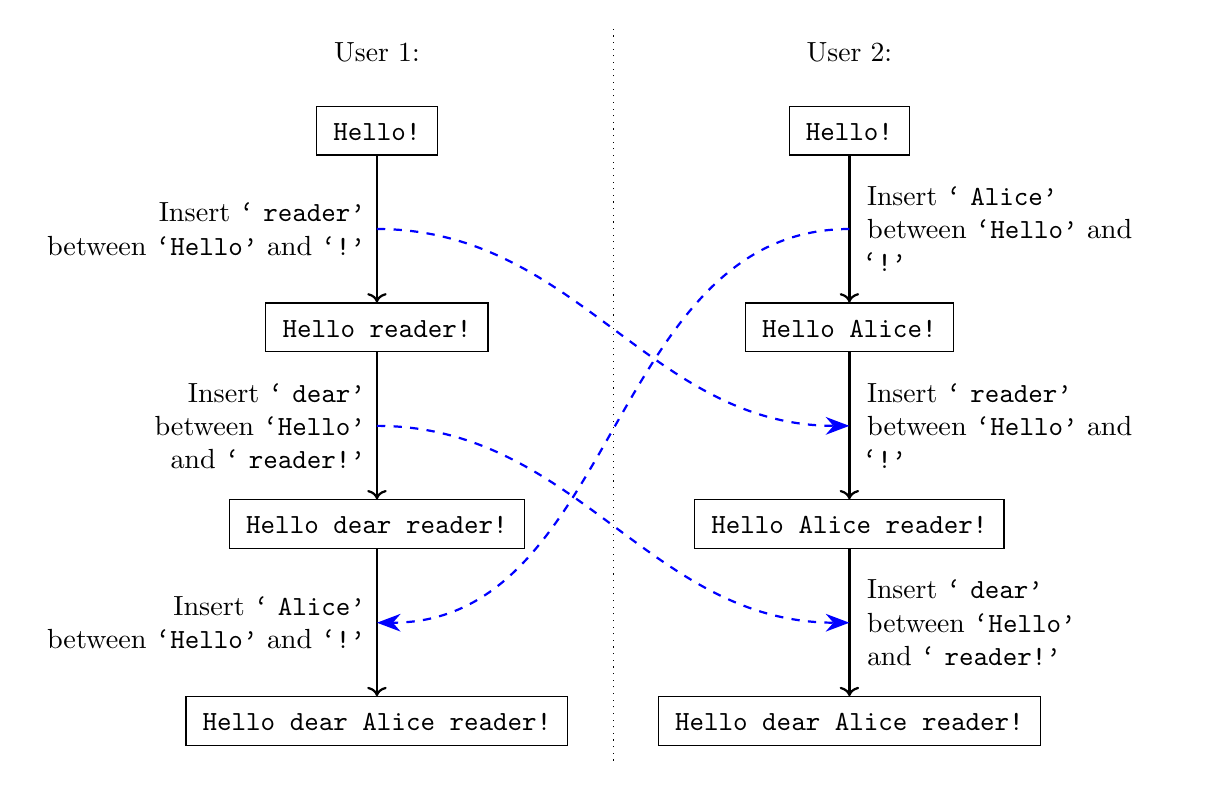
\begin{tikzpicture}[auto,scale=1.0]
    \tikzstyle{box}=[rectangle,draw,inner xsep=6pt,text height=9pt,text depth=2pt]
	\tikzstyle{leftevent}=[left,inner xsep=6pt,text width=4cm,text ragged left,midway]
	\tikzstyle{rightevent}=[right,inner xsep=6pt,text width=4cm,text ragged,midway]
	\tikzstyle{time}=[thick,->]
	\tikzstyle{network}=[thick,dashed,blue,-{Stealth[length=3mm]}]
	\node (left0)  at (0,8.5) {User 1:};
	\node (left1)  at (0,7.5) [box] {\texttt{Hello!}};
	\node (left2)  at (0,5.0) [box] {\texttt{Hello reader!}};
	\node (left3)  at (0,2.5) [box] {\texttt{Hello dear reader!}};
	\node (left4)  at (0,0.0) [box] {\texttt{Hello dear Alice reader!}};
	\node (right0) at (6,8.5) {User 2:};
	\node (right1) at (6,7.5) [box] {\texttt{Hello!}};
	\node (right2) at (6,5.0) [box] {\texttt{Hello Alice!}};
	\node (right3) at (6,2.5) [box] {\texttt{Hello Alice reader!}};
	\node (right4) at (6,0.0) [box] {\texttt{Hello dear Alice reader!}};
	\draw [time] (left1)  -- (left2)  node (send1) [leftevent]  {Insert \texttt{`~reader'}\\between \texttt{`Hello'} and \texttt{`!'}};
    \draw [time] (left2)  -- (left3)  node (send2) [leftevent]  {Insert \texttt{`~dear'}\\between \texttt{`Hello'}\\and \texttt{` reader!'}};
    \draw [time] (left3)  -- (left4)  node (recv3) [leftevent]  {Insert \texttt{`~Alice'}\\between \texttt{`Hello'} and \texttt{`!'}};
	\draw [time] (right1) -- (right2) node (send3) [rightevent] {Insert \texttt{`~Alice'}\\between \texttt{`Hello'} and \texttt{`!'}};
    \draw [time] (right2) -- (right3) node (recv1) [rightevent] {Insert \texttt{`~reader'}\\between \texttt{`Hello'} and \texttt{`!'}};
    \draw [time] (right3) -- (right4) node (recv2) [rightevent] {Insert \texttt{`~dear'}\\between \texttt{`Hello'}\\and \texttt{` reader!'}};
    \draw [network] (send1.east) to [out=0,in=180] (recv1.west);
    \draw [network] (send2.east) to [out=0,in=180] (recv2.west);
    \draw [network] (send3.west) to [out=180,in=0] (recv3.east);
	\path [draw,dotted] (3,-0.5) -- (3,8.8);
  \end{tikzpicture}
  \caption{The lesser interleaving anomaly that can occur with RGA.}
  \label{fig:rga-interleaving}
\end{figure*}

\begin{figure*}
  \centering
  \vspace{2em}
  \begin{tikzpicture}[auto,scale=1.0]
    \tikzstyle{box}=[rectangle,draw,inner xsep=6pt,text height=9pt,text depth=2pt]
    \node (head) at (2.5,6) [box] {\textit{head}};
	\node (hello1) at (4,6) [box] {\texttt{H}};
	\node (hello2) at (5,6) [box] {\texttt{e}};
	\node (hello3) at (6,6) [box] {\texttt{l}};
	\node (hello4) at (7,6) [box] {\texttt{l}};
	\node (hello5) at (8,6) [box] {\texttt{o}};
	\node (hello5t) at (8,6.6) {$\tau_0$};
	\node (hello6) at (12,4.2) [box] {\texttt{!}};
    \node (hello6t) at (12,3.6) {$\tau_1$};
    \node (dear1t) at (6,3.6) {$\tau_4$};
    \node (dear1)  at (6,4.2) [box] {\textit{space}};
	\node (dear2)  at (7,3) [box] {\texttt{d}};
	\node (dear3)  at (8,2) [box] {\texttt{e}};
	\node (dear4)  at (9,1) [box] {\texttt{a}};
	\node (dear5) at (10,0) [box] {\texttt{r}};
    \node (alice1t) at (8,3.6) {$\tau_3$};
    \node (alice1) at (8,4.2) [box] {\textit{space}};
	\node (alice2) at (9,3) [box] {\texttt{A}};
	\node (alice3) at (10,2) [box] {\texttt{l}};
	\node (alice4) at (11,1) [box] {\texttt{i}};
	\node (alice5) at (12,0) [box] {\texttt{c}};
	\node (alice6) at (13,-1) [box] {\texttt{e}};
    \node (reader1t) at (10,3.6) {$\tau_2$};
    \node (reader1) at (10,4.2) [box] {\textit{space}};
	\node (reader2) at (11,3) [box] {\texttt{r}};
	\node (reader3) at (12,2) [box] {\texttt{e}};
	\node (reader4) at (13,1) [box] {\texttt{a}};
	\node (reader5) at (14,0) [box] {\texttt{d}};
	\node (reader6) at (15,-1) [box] {\texttt{e}};
	\node (reader7) at (16,-2) [box] {\texttt{r}};
    \draw [->] (hello1) -- (head);
    \draw [->] (hello2) -- (hello1);
    \draw [->] (hello3) -- (hello2);
    \draw [->] (hello4) -- (hello3);
    \draw [->] (hello5) -- (hello4);
    \draw [->] (hello6.north west) -- (hello5.east);
    \draw [->] (dear1) -- (hello5.south west);
    \draw [->] (dear2.north west) -- (dear1.south east);
    \draw [->] (dear3) -- (dear2);
    \draw [->] (dear4) -- (dear3);
    \draw [->] (dear5) -- (dear4);
    \draw [->] (alice1) -- (hello5.south);
    \draw [->] (alice2.north west) -- (alice1.south east);
    \draw [->] (alice3) -- (alice2);
    \draw [->] (alice4) -- (alice3);
    \draw [->] (alice5) -- (alice4);
    \draw [->] (alice6) -- (alice5);
    \draw [->] (reader1) -- (hello5.south east);
    \draw [->] (reader2.north west) -- (reader1.south east);
    \draw [->] (reader3) -- (reader2);
    \draw [->] (reader4) -- (reader3);
    \draw [->] (reader5) -- (reader4);
    \draw [->] (reader6) -- (reader5);
    \draw [->] (reader7) -- (reader6);
  \end{tikzpicture}
  \caption{The tree structure underlying the RGA example in Figure~\ref{fig:rga-interleaving}: each node
  represents a character, and its parent is the immediate predecessor character at the time it was inserted.
  The document state corresponds to a depth-first pre-order traversal over this tree, with sibling nodes
  visited in descending timestamp order ($\tau_4 > \tau_3 > \tau_2 > \tau_1$).}
  \label{fig:rga-tree}
\end{figure*}

\section{The lesser interleaving anomaly}\label{sec:lesser}

The RGA algorithm for collaborative text editing~\cite{Roh:2011dw} does not suffer from the anomaly described in Section~\ref{sec:anomaly}, as we proved in prior work~\cite{ExtendedVersion,AFP}.
In particular, if the insertions are made in sequential order (e.g. the string \texttt{` Alice'} is inserted by first typing a space, then the letter \texttt{`A'}, then the letter \texttt{`l'}, etc.), then RGA guarantees that there will be no interleaving.
In the scenario of Figure~\ref{fig:bad-merge}, assuming sequential insertions, RGA allows only two possible outcomes of the merge: either \texttt{`Hello Alice Charlie!'} or \texttt{`Hello Charlie Alice!'} with no mixture of the two permitted.

However, RGA does not satisfy the revised specification of Section~\ref{sec:attiya-spec} because it allows a lesser anomaly: text may be interleaved if insertions are not sequential.
This lesser anomaly is illustrated in Figure~\ref{fig:rga-interleaving}.
In this example, User 1 first positions the cursor between \texttt{`Hello'} and the exclamation mark, types the word \texttt{` reader'}, then \emph{moves the cursor back} to a position immediately after \texttt{`Hello'}, and types the word \texttt{` dear'}.

In RGA an insertion is anchored to the existing character that immediately precedes the character to be inserted.
Thus, in Figure~\ref{fig:rga-interleaving}, the first character of \texttt{` reader'} and the first character of \texttt{` dear'} are both anchored to the last character of \texttt{`Hello'}.
When User 2 makes a concurrent insertion of \texttt{` Alice'}, it is also anchored to the last character of \texttt{`Hello'}.
This tree of anchoring relationships is illustrated in Figure~\ref{fig:rga-tree} (Attiya et al. call this structure a \emph{timestamped insertion tree}~\cite{Attiya:2016kh}, while Grishchenko calls it a \emph{causal tree}~\cite{Grishchenko:2014eh}).

When multiple insertions are anchored to the same character, they are sorted in descending timestamp order.
In the example, we can assume that the timestamp of the insertion of \texttt{` dear'} is greater than that of \texttt{` reader'}, since these insertions were performed sequentially by the same user.
However, we do not know the timestamp of \texttt{` Alice'} relative to the other two insertions, and hence that insertion can be ordered arbitrarily relative to other insertions with the same anchor.
Thus, in this example, RGA allows three possible outcomes of the merge:

\begin{enumerate}
\item \texttt{`Hello dear reader Alice!'}
\item \texttt{`Hello dear Alice reader!'}
\item \texttt{`Hello Alice dear reader!'}
\end{enumerate}

Although RGA rules out random character-by-character interleaving, it does still allow the word \texttt{`Alice'} to be interleaved between the two insertion sequences by User 1.
We characterise this as a lesser form of the anomaly described in Section~\ref{sec:anomaly}.

The worst case for RGA occurs if the user types all characters in the reverse order of their appearance in the document, i.e.\ the document is typed back to front.
In this case, all characters would be anchored to the head of the document, ordered only by timestamp, and thus arbitrary character-level interleaving could occur.
Whilst this editing pattern is unlikely to occur in realistic editing scenarios, it is a case that must be considered by formal consistency models for collaborative text editors.

\subsection{Fixing interleaving in RGA}\label{sec:fixing-rga}

RGA assigns a unique logical timestamp to every operation, and treats that timestamp as the identifier for that operation.
Roh et al.'s original definition of RGA used a custom S4Vector datatype as timestamp~\cite{Roh:2011dw}, and subsequent presentations of the algorithm~\cite{Shapiro:2011wy} have used Lamport timestamps~\cite{Lamport:1978jq} instead.
Our RGA fix works by changing the algorithm to use a new timestamp definition.

In Attiya et al.'s formulation of RGA~\cite{Attiya:2016kh}, an insertion operation is represented by a triple $(a, t, r)$ where $a$ is the character being inserted, $t$ is the timestamp of the operation, and $r$ is the timestamp of the \emph{reference character} (the timestamp of the operation that inserted the immediate predecessor character at the time the insertion was performed, or the distinguished value \textit{head} if the insertion was performed at the beginning of the document).
Deletion operations are performed by marking a character as deleted but retaining its position in the document as a \emph{tombstone}.
Since deletions do not affect identifier order in the document, we ignore them henceforth.

We extend this definition to represent each insertion operation by a 4-tuple $(a, t, r, e)$ where $a$, $t$ and $r$ are defined as before, and $e$ is the set of timestamps of all insertion operations with the same reference character $r$ at the time the insertion was performed (not including $t$ itself).
Let $I$ be the set of insertion operations that have been performed on a document at a given point in time.
To insert a character $a$ after reference character $r$ in this document, we create a new timestamp $t$, create an insertion operation, and add it to $I$:
\[ I' = I \;\cup\; \big\{\,(a,\, t,\, r,\, \{t' \mid \exists a', e'.\; (a', t', r, e') \in I \}\,)\,\big\} \]

In the example of Figure~\ref{fig:rga-tree}, if the timestamp of the last character of \texttt{`Hello'} is $\tau_0$, the set of insertions contains $(\texttt{`!'}, \tau_1, \tau_0, \{\})$ for the exclamation mark, $(\texttt{`~'}, \tau_2, \tau_0, \{\tau_1\})$ for the first character of \texttt{`~reader'}, $(\texttt{`~'}, \tau_3, \tau_0, \{\tau_1\})$ for the first character of \texttt{`~Alice'}, and $(\texttt{`~'}, \tau_4, \tau_0, \{\tau_1, \tau_2\})$ for the first character of \texttt{`~dear'}.

In order to use this insertion 4-tuple in RGA we need to define a total order that is used to sort insertions with the same reference character.
Consider two distinct insertion operations $\mathit{ins}_1$ and $\mathit{ins}_2$ with the same reference character $r$:
\[ \mathit{ins}_1 = (a_1, t_1, r, e_1) \quad\text{and}\quad \mathit{ins}_2 = (a_2, t_2, r, e_2). \]
First observe that if $\mathit{ins}_1$ happened before $\mathit{ins}_2$ we must have $t_1 \in e_2$, and vice versa.
In this case we make the ordering of operations consistent with the \emph{happens-before} relation:
\begin{align*}
(a_1, t_1, r, e_1) < (a_2, t_2, r, e_2) &\quad\text{if } t_1 \in e_2 \\
(a_2, t_2, r, e_2) < (a_1, t_1, r, e_1) &\quad\text{if } t_2 \in e_1
\end{align*}
Otherwise $\mathit{ins}_1$ and $\mathit{ins}_2$ are concurrent, and we have $t_1 \notin e_2$ and $t_2 \notin e_1$.
From this we can deduce that
\[ \{t_1\} \cup e_1 - e_2 \ne \{\} \quad\text{and}\quad \{t_2\} \cup e_2 - e_1 \ne \{\}. \]
As these sets are nonempty and we have a total ordering on timestamps, each of them has a unique minimal element:
\[ m_1 = \mathrm{min}(\{t_1\} \cup e_1 - e_2) \quad\text{and}\quad m_2 = \mathrm{min}(\{t_2\} \cup e_2 - e_1) \]
The timestamps $m_1$ and $m_2$ identify the first operations at which the editing histories of $\mathit{ins}_1$ and $\mathit{ins}_2$ diverged.
From the definition above it follows that $m_1 \ne m_2$.
We can now define the ordering of concurrent operations based on the relative ordering of $m_1$ and $m_2$:
\begin{align*}
(a_1, t_1, r, e_1) < (a_2, t_2, r, e_2) &\quad\text{if } m_1 < m_2 \\
(a_2, t_2, r, e_2) < (a_1, t_1, r, e_1) &\quad\text{if } m_2 < m_1
\end{align*}
This order has the property that all of the operations in a particular editing session are grouped, so that they are either all less than or all greater than the operations in a different, concurrent editing session.
Hence, all characters inserted during a particular editing session are grouped together in the final document, and interleaving of insertions from concurrent editing sessions is prevented.
We conjecture that applying this construction to RGA results in a CRDT without interleaving, as required by our specification in Section~\ref{sec:attiya-spec}.
A formal proof of this conjecture is left for future work.

Our construction increases the memory and network bandwidth used by the CRDT, due to the additional timestamp set $e$ that needs to be included in each operation.
However, the sets are expected to be small, since there are normally not many operations with the same reference character, regardless of the length of the document.

\section{Conclusions}

Several published CRDT algorithms for collaborative text editing exhibit an undesirable anomaly in which concurrently inserted portions of text may be randomly interleaved on a character-by-character basis, resulting in an unreadable jumble of letters.
We highlighted two cases of undesirable interleaving, one affecting Logoot and LSEQ, and the other affecting RGA.

The interleaving anomaly in Logoot and LSEQ has been independently pointed out in our draft manuscript~\cite{ExtendedVersion}, by Sun et al.~\cite{Sun:2018wb}, and by a Stack Overflow user~\cite{StackOverflowInterleaving}.
From conversations with various members of the CRDT community it appears that the anomaly has been known in the community folklore for some time, but to our knowledge there is no published work that clearly explains the problem or proposes solutions.

In this paper we proposed an improved specification of collaborative text editing that rules out these interleaving anomalies, and proposed a modification to the RGA algorithm that, we conjecture, rules out the interleaving anomaly in this algorithm.

\begin{acks}
This work was supported by The Boeing Company and the EPSRC ``REMS: Rigorous Engineering for Mainstream Systems'' programme grant (EP/K008528).
\end{acks}

\bibliographystyle{ACM-Reference-Format}
\bibliography{references}
\end{document}
